% Provenance (never printed): see sources/outline_sources.md (Year 3:
% dislocation and diffusion creep; flow laws; deformation maps; shear zones and
% kinematic indicators). Brief: sources/book5/BRIEFS.md, ch. 7. Curves from
% figdata/bachelor-3/flow_laws.py. Exercise and problem values in the Book 5
% scratch calculator calc/ch07.py.
\chapter{Mekanisme Deformasi dan Zona Geser}\label{ch:b3:deformation-mechanisms}

Di permukaan, granit sebuah gunung pecah sepanjang sesar-sesar.
Dua puluh kilometer ke bawah, granit yang sama mengalir seperti dodol dalam \omterm{def:b3:deformation-mechanisms:shear-zone}{zona geser} yang lebarnya
hanya beberapa ratus meter, feldsparnya tergilas menjadi mata dan kuarsanya tertarik memanjang
menjadi pita. Kristal dapat mengalir tanpa patah karena kristal tidak pernah sempurna:
ia bergerak melalui cacatnya, satu baris atom pada satu waktu, atau melalui atom yang
berdifusi dari satu sisi butir ke sisi lain. Bab ini mengikuti mekanisme-mekanisme tersebut dari kisi
kristal hingga hukum-hukum yang dipakai geodinamika, ke peta yang menunjukkan mekanisme mana yang
dominan, dan ke \omterm{def:b3:deformation-mechanisms:shear-zone}{zona geser} tempat batuan mencatat bagaimana ia bergerak.

\begin{recall}
Cacat titik, hukum Arrhenius, dan energi aktivasi dibahas dalam
volume universitas buku kimia; koefisien difusi dalam
buku fisika. Tegangan dan regangan, elips regangan, geser sederhana, dan elipsnya
($S_{1,2} = \sqrt{1 + \gamma^2/4} \pm \gamma/2$, sumbu panjang pada $\theta'$ dari
\omterm{def:b3:deformation-mechanisms:kinematic}{arah geser} dengan $\tan2\theta' = 2/\gamma$), rayapan hukum pangkat dengan
konstantanya untuk kuarsit basah dan olivin kering, selubung kekuatan, serta
transisi getas--liat dibahas dalam volume Tahun 1, pada bab tentang
tegangan, regangan, dan reologi; foliasi, lineasi, dan
milonit deskriptif pada bab tentang sesar, lipatan, dan fabrik. Viskositas efektif
mantel ada pada \cref{ch:b3:mantle-convection}.
\end{recall}

\section{Cacat kristal}

Untuk menggeser kristal sempurna, setiap ikatan yang melintasi bidang kisi harus
putus sekaligus, dan itu memerlukan tegangan sekitar sepersepuluh modulus geser,
yang di mantel kira-kira \qty{8e10}{Pa}
(\cref{ch:b3:mantle-convection}): ribuan megapascal. Kristal nyata mulai luluh
pada tegangan jauh lebih rendah, karena mereka tergelincir satu baris atom pada satu waktu.

\begin{definition}[Dislokasi]\label{def:b3:deformation-mechanisms:dislocation}
Yang disebut \emph{dislokasi}\index{dislokasi (cacat kristal)} adalah cacat garis dalam
kristal: batas di dalam kristal antara bagian bidang kisi yang telah tergelincir
dan bagian yang belum. Vektor \emph{vektor Burgers}-nya
$\mathbf b$ adalah pergeseran yang dibawanya, sebesar satu jarak kisi dalam
arah kisi. Pada dislokasi tepi, $\mathbf b$ tegak lurus terhadap garis,
yakni tepi setengah bidang atom tambahan; pada dislokasi sekrup ia
sejajar dengan garis. Dislokasi bergerak dengan \emph{gelincir} pada bidang gelincirnya,
dan dislokasi tepi meninggalkan bidang itu dengan \emph{pendakian}, saat atom atau
kekosongan berdifusi ke atau dari tepi setengah bidangnya.
\end{definition}

\begin{omfigure}
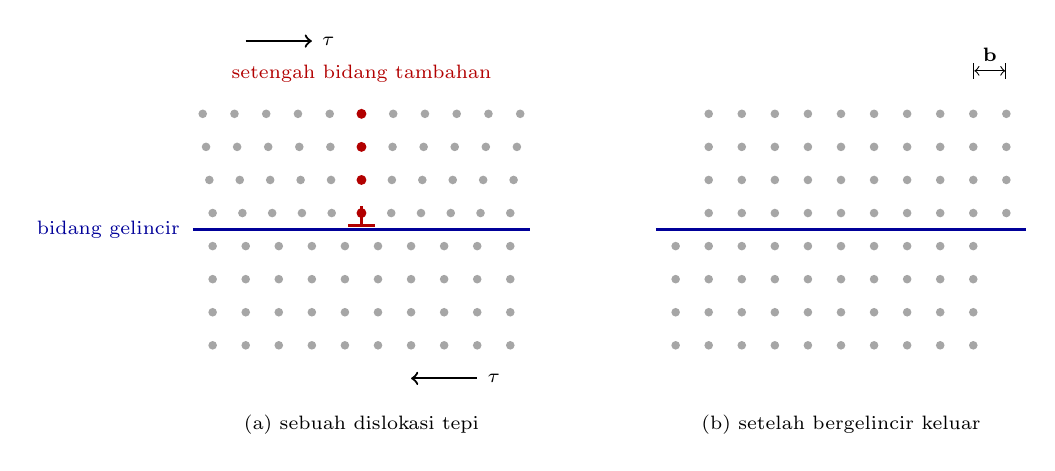
\begin{tikzpicture}[font=\scriptsize, x=0.42cm, y=0.42cm]
% (a) lower half: 10 columns; upper half: 11 columns squeezed over the same width
\foreach \j in {0,...,3} {\foreach \i in {0,...,9} {\fill[gray!70] (\i,\j) circle (0.13);}}
\foreach \j/\s in {4/0.9, 5/0.92, 6/0.94, 7/0.96} {\foreach \i in {0,...,10} {
  \pgfmathsetmacro{\x}{(\i-5)*\s + 4.5}
  \ifnum\i=5 \fill[red!70!black] (\x,\j) circle (0.15); \else \fill[gray!70] (\x,\j) circle (0.13); \fi}}
\draw[thick, blue!60!black] (-0.6,3.5) -- (9.6,3.5);
\node[anchor=east, blue!60!black] at (-0.7,3.5) {bidang gelincir};
\draw[red!70!black, very thick] (4.1,3.62) -- (4.9,3.62) (4.5,3.62) -- (4.5,4.2);
\node[red!70!black] at (4.5,8.2) {setengah bidang tambahan};
\draw[->, thick] (1.0,9.2) -- (3.0,9.2) node[right] {$\tau$};
\draw[<-, thick] (6.0,-1.0) -- (8.0,-1.0) node[right] {$\tau$};
% (b) after glide: the upper half shifted by one spacing
\begin{scope}[shift={(14,0)}]
\foreach \j in {0,...,3} {\foreach \i in {0,...,9} {\fill[gray!70] (\i,\j) circle (0.13);}}
\foreach \j in {4,...,7} {\foreach \i in {1,...,10} {\fill[gray!70] (\i,\j) circle (0.13);}}
\draw[thick, blue!60!black] (-0.6,3.5) -- (10.6,3.5);
\draw[|<->|] (9,8.3) -- (10,8.3) node[midway, above] {$\mathbf b$};
\end{scope}
\node[anchor=north] at (4.5,-1.8) {(a) sebuah dislokasi tepi};
\node[anchor=north] at (19,-1.8) {(b) setelah bergelincir keluar};
\end{tikzpicture}

\par\smallskip{\small (a) Sebuah \omterm{def:b3:deformation-mechanisms:dislocation}{dislokasi} tepi: setengah bidang atom tambahan (merah)
berakhir pada bidang gelincir, sehingga mendistorsi kisi di sekitar tepinya (simbol
$\perp$). Di bawah tegangan geser $\tau$, ia bergelincir sepanjang bidang gelincir dengan
memutus dan membentuk kembali satu baris ikatan pada satu waktu. (b) Setelah ia
melintasi kristal, bagian atas telah tergeser sebesar satu vektor Burgers $\mathbf b$, dan
kisinya kembali sempurna.}\label{fig:b3:deformation-mechanisms:dislocation}
\end{omfigure}

Kisi menahan gelincir \omterm{def:b3:deformation-mechanisms:dislocation}{dislokasi} dengan tegangan kecil, yaitu
tegangan Peierls, yang bergantung pada kekuatan dan arah ikatan:
itulah sebabnya beberapa sistem gelincir mineral mudah dan yang lain sulit. Ketika
kristal berdeformasi, \omterm{def:b3:deformation-mechanisms:dislocation}{dislokasi} berlipat ganda dan saling kusut; mereka saling menghalangi, dan
kristal mengeras, kecuali jika mereka dapat memanjat melewati rintangan atau saling meniadakan, yang
membutuhkan difusi, dan karena itu panas.

\section{Mekanisme rayapan}

\begin{definition}[Mekanisme rayapan]\label{def:b3:deformation-mechanisms:creep}
Pada \emph{rayapan dislokasi}\index{rayapan dislokasi} kristal berdeformasi melalui
gelincir \omterm{def:b3:deformation-mechanisms:dislocation}{dislokasi}, dengan pendakian yang melepaskannya dari rintangan. Pada
\emph{rayapan difusi}\index{rayapan difusi} kristal mengubah bentuk melalui
difusi atom, melalui kisi (rayapan Nabarro--Herring) atau sepanjang
batas butir (rayapan Coble), dari sisi yang berada di bawah tegangan normal tertinggi
menuju sisi yang berada di bawah tegangan terendah. Pada \emph{gelincir batas butir}\index{gelincir batas butir}
butir-butir meluncur melewati satu sama lain sepanjang batasnya, dengan celah yang
ditutup oleh difusi atau rayapan \omterm{def:b3:deformation-mechanisms:dislocation}{dislokasi}. Pada \emph{pelarutan
tekanan}\index{pelarutan tekanan} materi larut dalam lapisan fluida pada sisi yang
berada di bawah tegangan tinggi dan diendapkan di tempat tegangannya rendah, atau terbawa
pergi.
\end{definition}

\begin{proposition}[Ketergantungan ukuran butir pada rayapan difusi]\label{prop:b3:deformation-mechanisms:grain-size}
Pada tegangan rendah $\sigma$, batuan dengan ukuran butir $d$ merayap secara difusi dengan laju
\[
  \dot\varepsilon \approx B_L\frac{D_L\Omega}{k_BT}\frac{\sigma}{d^2}
  \quad\text{(melalui kisi)},\qquad
  \dot\varepsilon \approx B_B\frac{\delta D_B\Omega}{k_BT}\frac{\sigma}{d^3}
  \quad\text{(sepanjang batas)},
\]
dengan $D_L$ dan $D_B$ adalah koefisien difusi di dalam kisi dan di
batas, $\delta$ lebar batas, $\Omega$ volume satu atom,
$k_B$ konstanta Boltzmann, dan $B_L$, $B_B$ bilangan berorde sepuluh yang bergantung pada
bentuk butirnya.
\end{proposition}

\begin{proof}
Tegangan normal $\sigma$ pada suatu bidang mengubah kerja yang diperlukan untuk membentuk satu kekosongan
di sana sebesar $\sigma\Omega$, sehingga konsentrasi $C$ kekosongan berbeda antara
bidang yang mengalami tarikan dan yang mengalami tekanan, sebesar $\Delta C \approx C\sigma\Omega/
(k_BT)$ ketika $\sigma\Omega \ll k_BT$. Melintasi jarak berorde $d$, fluks
difusif kekosongan, dan dengan demikian juga fluks atom ke arah sebaliknya, berorde $D\Delta
C/d$ per satuan luas. Melalui kisi, fluks melintasi luas berorde
$d^2$, sepanjang batas luas berorde $\delta d$. Volume yang berpindah per
satuan waktu, dibagi volume butir $d^3$, adalah laju regangan: berorde
$(D_L\sigma\Omega/k_BT)\,d^2/(d\cdot d^3) = D_L\sigma\Omega/(k_BTd^2)$ di dalam
kisi, dan $(D_B\sigma\Omega/k_BT)\,\delta d/(d\cdot d^3) = \delta D_B
\sigma\Omega/(k_BTd^3)$ di dalam batas. Hasil kali $C\,D$ adalah
koefisien difusi-diri yang ditulis $D$ dalam pernyataan.
\end{proof}

\omterm{def:b3:deformation-mechanisms:creep}{Rayapan difusi} linear terhadap tegangan, berupa aliran viskos sejati, dan berlangsung cepat pada
batuan berbutir halus: memperkecil ukuran butir menjadi separuh membuat rayapan Coble delapan kali lebih cepat
(gambar di bawah). \omterm{def:b3:deformation-mechanisms:creep}{Rayapan dislokasi} tidak bergantung pada ukuran butir, tetapi meningkat
dengan pangkat tinggi terhadap tegangan.

\begin{omfigure}
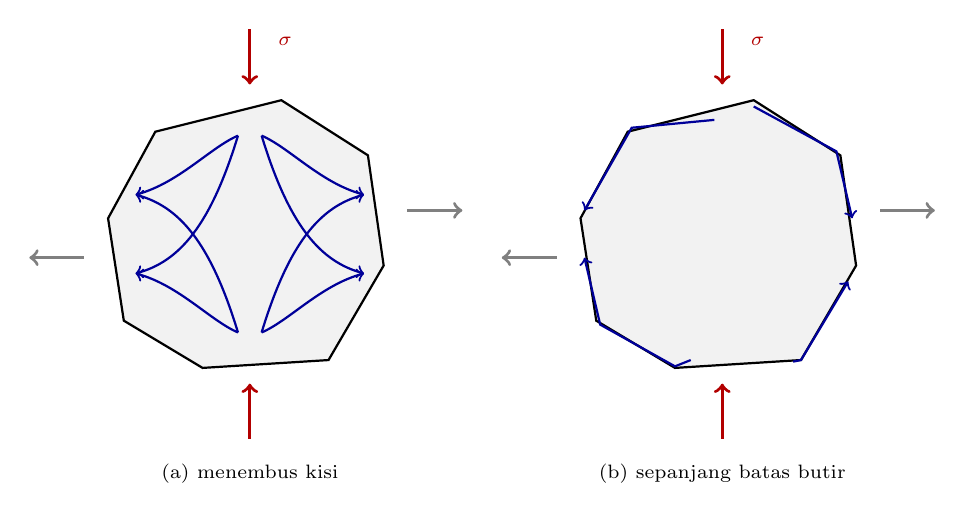
\begin{tikzpicture}[font=\scriptsize, x=1cm, y=1cm]
\foreach \cx/\lab in {0/{(a) menembus kisi}, 6/{(b) sepanjang batas butir}} {
  \begin{scope}[shift={(\cx,0)}]
  \draw[thick, fill=gray!10] (-1.6,-1.1) -- (-0.6,-1.7) -- (1.0,-1.6) -- (1.7,-0.4) -- (1.5,1.0) -- (0.4,1.7) -- (-1.2,1.3) -- (-1.8,0.2) -- cycle;
  \draw[->, very thick, red!70!black] (0,2.6) -- (0,1.9);
  \draw[->, very thick, red!70!black] (0,-2.6) -- (0,-1.9);
  \node[red!70!black] at (0.45,2.45) {$\sigma$};
  \draw[<-, very thick, gray] (2.7,0.3) -- (2.0,0.3);
  \draw[<-, very thick, gray] (-2.8,-0.3) -- (-2.1,-0.3);
  \node[anchor=north] at (0,-2.8) {\lab};
  \end{scope}
}
\foreach \sx in {1,-1} {\foreach \y in {-0.5,0.5} {
  \draw[->, blue!60!black, thick] (0.15*\sx,1.25) .. controls (0.5*\sx,\y+0.6) and (0.9*\sx,\y+0.15) .. (1.45*\sx,\y);
  \draw[->, blue!60!black, thick] (0.15*\sx,-1.25) .. controls (0.5*\sx,\y-0.6) and (0.9*\sx,\y-0.15) .. (1.45*\sx,\y);
}}
\draw[->, blue!60!black, thick] (6.4,1.62) -- (7.45,1.05) -- (7.65,0.2);
\draw[->, blue!60!black, thick] (5.9,1.45) -- (4.85,1.35) -- (4.25,0.3);
\draw[->, blue!60!black, thick] (6.9,-1.62) -- (7.0,-1.6) -- (7.6,-0.6);
\draw[->, blue!60!black, thick] (5.6,-1.6) -- (5.4,-1.68) -- (4.45,-1.15) -- (4.25,-0.3);
\end{tikzpicture}

\par\smallskip{\small \omterm{def:b3:deformation-mechanisms:creep}{Rayapan difusi} pada butir yang memendek sepanjang $\sigma$. Atom
meninggalkan permukaan yang mengalami kompresi tertinggi dan ditambahkan ke permukaan yang mengalami
kompresi terendah (biru), sehingga butir menjadi gepeng dan memanjang (panah abu-abu): (a)
melalui bagian dalam butir, rayapan Nabarro--Herring; (b) sepanjang batasnya,
rayapan Coble.}\label{fig:b3:deformation-mechanisms:diffusion}
\end{omfigure}

Kristal yang terdeformasi juga memperbaiki diri sendiri selama ia mengalami deformasi.

\begin{definition}[Pemulihan, subbutir, rekristalisasi dinamis]\label{def:b3:deformation-mechanisms:recrystallisation}
Yang disebut \emph{pemulihan}\index{pemulihan (plastisitas kristal)} adalah penataan ulang
\omterm{def:b3:deformation-mechanisms:dislocation}{dislokasi}, melalui pemanjatan dan silang-geser, menjadi susunan berenergi lebih rendah, serta
pemusnahannya. \omterm{def:b3:deformation-mechanisms:dislocation}{Dislokasi} yang tersusun dalam dinding membagi sebuah butir menjadi
\emph{subbutir}\index{subbutir}, yaitu bagian butir yang kisinya miring
beberapa derajat satu sama lain. \emph{rekristalisasi
dinamis}\index{rekristalisasi dinamis} adalah penggantian butir yang tertegang selama
deformasi oleh butir baru dengan \omterm{def:b3:deformation-mechanisms:dislocation}{dislokasi} lebih sedikit, baik
melalui rotasi subbutir hingga menjadi butir, atau melalui migrasi
batas butir masuk ke tetangga yang lebih tegang.
\end{definition}

\begin{definition}[Orientasi kristalografi terpilih]\label{def:b3:deformation-mechanisms:cpo}
Dikatakan bahwa batuan memiliki \emph{orientasi kristalografi terpilih}\index{orientasi kristalografi terpilih}
(CPO) ketika kisi-kisi butirnya tidak berorientasi
acak, melainkan mengelompok di sekitar arah yang ditentukan oleh deformasi; \omterm{def:b3:deformation-mechanisms:creep}{rayapan dislokasi}
menghasilkannya, dengan memutar sistem geser tiap butir menuju arah aliran.
\end{definition}

Batuan dengan CPO mewarisi anisotropi kristalnya: kecepatan seismiknya,
misalnya, bergantung pada arah, sehingga seismologi dapat melihat fabrik
mantel dalam. \omterm{def:b3:deformation-mechanisms:creep}{Rayapan difusi} dan \omterm{def:b3:deformation-mechanisms:creep}{gelincir batas butir}, yang membiarkan butir
berotasi dengan bebas, tidak membentuknya.

\section{Hukum aliran}

\begin{definition}[Hukum aliran, eksponen tegangan, suhu homolog]\label{def:b3:deformation-mechanisms:flow-law}
Yang disebut \emph{hukum aliran}\index{hukum aliran} memberikan laju regangan batuan yang mengalami deformasi oleh
satu mekanisme sebagai fungsi tegangan diferensial $\sigma$, ukuran butir
$d$, suhu $T$, dan tekanan $P$:
\[
  \dot\varepsilon = A\,\sigma^nd^{-m}\exp\Bigl(-\frac{E + PV}{RT}\Bigr),
\]
dengan $A$, $n$, $m$, energi aktivasi $E$, dan volume aktivasi $V$
diukur di laboratorium. \emph{Eksponen tegangan}\index{eksponen tegangan}
adalah $n$, dan eksponen ukuran butir $m$. \emph{Suhu
homolog}\index{suhu homolog} suatu mineral adalah $T/T_m$, yaitu
suhu absolutnya dibagi suhu lelehnya dalam skala absolut.
\end{definition}

Dalam hukum yang digunakan di sini, \omterm{def:b3:deformation-mechanisms:creep}{rayapan dislokasi} memiliki $n$ sebesar 3.5 atau 4 dan $m = 0$;
\omterm{def:b3:deformation-mechanisms:creep}{rayapan difusi} memiliki $n = 1$ dan $m = 2$ atau 3 (lihat \cref{prop:b3:deformation-mechanisms:grain-size}).
Rayapan meningkat ketika \omterm{def:b3:deformation-mechanisms:flow-law}{suhu homolog} mendekati 1. Forsterit meleleh pada \qty{1890}{\celsius}, sehingga mantel pada \qty{1300}{\celsius}
berada pada $T/T_m = 0.73$; es pada \qty{-10}{\celsius} pada 0.96, itulah sebabnya
gletser mengalir. Nilai olivin yang dipakai di sini berasal dari
kompilasi laboratorium yang banyak digunakan: olivin kering dalam \omterm{def:b3:deformation-mechanisms:creep}{rayapan dislokasi}, $A =
\num{1.1e5}$, $n = 3.5$, $E = \qty{530}{kJ.mol^{-1}}$, $V =
\qty{14}{cm^3.mol^{-1}}$; dalam \omterm{def:b3:deformation-mechanisms:creep}{rayapan difusi}, $A = 10^{9.2}$, $n = 1$, $m = 3$,
$E = \qty{375}{kJ.mol^{-1}}$, $V = \qty{5}{cm^3.mol^{-1}}$ (tegangan dalam megapaskal,
ukuran butir dalam mikrometer, waktu dalam detik); kuarsit basah dibahas
dalam volume Tahun 1. Air melemahkan olivin: pada fugasitas air sekitar
\qty{300}{MPa}, agregat olivin merayap lima hingga enam kali lebih cepat daripada yang kering
dalam \omterm{def:b3:deformation-mechanisms:creep}{rayapan dislokasi}, dan lima kali lebih cepat dalam \omterm{def:b3:deformation-mechanisms:creep}{rayapan difusi}.
% ledger: bowen14:mgo-sio2, azuma17:olivine, lopez:flow-laws, codata:R, mk00:diffusion, mk00:dislocation

\begin{proposition}[Viskositas efektif]\label{prop:b3:deformation-mechanisms:viscosity}
Batuan yang mematuhi \omterm{def:b3:deformation-mechanisms:flow-law}{hukum aliran} $\dot\varepsilon = A'\sigma^n$ pada $T$, $P$, dan
$d$ yang diberikan memiliki viskositas efektif
\[
  \eta_{\mathrm{eff}} = \frac{\sigma}{2\dot\varepsilon}
  = \tfrac12A'^{-1/n}\,\dot\varepsilon^{(1-n)/n}:
\]
untuk $n > 1$ ia turun seiring batuan mengalami deformasi lebih cepat.
\end{proposition}

\begin{proof}
Untuk fluida Newton, $\sigma = 2\eta\dot\varepsilon$ pada aliran uniaksial, berdasarkan
definisi viskositas; $\eta_{\mathrm{eff}}$ adalah viskositas fluida Newton yang
akan mengalir dengan laju yang sama di bawah tegangan yang sama. Dengan mensubstitusikan
$\sigma = (\dot\varepsilon/A')^{1/n}$ diperoleh bentuk kedua.
\end{proof}

Kuarsit basah pada \qty{400}{\celsius} yang mengalir dengan laju \qty{e-14}{s^{-1}} membutuhkan
\qty{65}{MPa} dan memiliki viskositas efektif sebesar \qty{3.3e21}{Pa.s}; pada
\qty{500}{\celsius}, \qty{18}{MPa} dan \qty{9e20}{Pa.s}: kenaikan seratus derajat
memangkas kekuatannya lebih dari tiga kali lipat (gambar di bawah). Olivin kering pada
\qty{1100}{\celsius} dan \qty{1}{GPa} hanya membutuhkan \qty{3}{MPa}. Amplop kekuatan
pada volume Tahun 1 dibangun tepat dari hukum-hukum ini.

\begin{omfigure}
\begin{tikzpicture}
\begin{groupplot}[group style={group size=2 by 1, horizontal sep=1.6cm},
  omrecord, width=0.47\linewidth, height=0.47\linewidth, xmode=log,
  xmin=1, xmax=1000, ymin=-20, ymax=-6, xlabel={tegangan diferensial (MPa)},
  legend style={font=\scriptsize, at={(0.97,0.03)}, anchor=south east, legend columns=1}]
\nextgroupplot[ylabel={$\log_{10}\dot\varepsilon$ (\unit{s^{-1}})}, title={(a) kuarsit basah},
  title style={font=\small}]
% computed in figdata/bachelor-3/flow_laws.py; ledger: lopez:flow-laws, azuma17:olivine
\addplot[omDef, thick] table[x=s, y=r600] {figdata/out/bachelor-3-flow_laws-quartz.dat};
\addlegendentry{\qty{600}{\celsius}}
\addplot[red!70!black, thick, densely dashed] table[x=s, y=r500] {figdata/out/bachelor-3-flow_laws-quartz.dat};
\addlegendentry{\qty{500}{\celsius}}
\addplot[black, thick, densely dotted] table[x=s, y=r400] {figdata/out/bachelor-3-flow_laws-quartz.dat};
\addlegendentry{\qty{400}{\celsius}}
\draw[gray] (axis cs:1,-14) -- (axis cs:1000,-14);
\nextgroupplot[title={(b) olivin kering, \qty{1}{GPa}}, title style={font=\small}]
\addplot[omDef, thick] table[x=s, y=r1300] {figdata/out/bachelor-3-flow_laws-olivine.dat};
\addlegendentry{\qty{1300}{\celsius}}
\addplot[red!70!black, thick, densely dashed] table[x=s, y=r1100] {figdata/out/bachelor-3-flow_laws-olivine.dat};
\addlegendentry{\qty{1100}{\celsius}}
\addplot[black, thick, densely dotted] table[x=s, y=r900] {figdata/out/bachelor-3-flow_laws-olivine.dat};
\addlegendentry{\qty{900}{\celsius}}
\draw[gray] (axis cs:1,-14) -- (axis cs:1000,-14);
\end{groupplot}
\end{tikzpicture}

\par\smallskip{\small \omterm{def:b3:deformation-mechanisms:flow-law}{Hukum aliran} \omterm{def:b3:deformation-mechanisms:creep}{rayapan dislokasi}: laju regangan terhadap tegangan pada
tiga suhu. Kemiringan pada sumbu ini adalah \omterm{def:b3:deformation-mechanisms:flow-law}{eksponen tegangan}, 4 untuk
kuarsit dan 3.5 untuk olivin; garis abu-abu menandai laju regangan geologi,
\qty{e-14}{s^{-1}}. Olivin membutuhkan suhu sekitar \qty{600}{\celsius} lebih tinggi
daripada kuarsa agar dapat mengalir semudah itu.}\label{fig:b3:deformation-mechanisms:flow-laws}
\end{omfigure}

\section{Peta mekanisme deformasi}

Beberapa mekanisme berlangsung secara paralel, dan yang tercepat menentukan deformasinya.

\begin{definition}[Peta mekanisme deformasi]\label{def:b3:deformation-mechanisms:deformation-map}
Sebuah \emph{peta mekanisme deformasi}\index{peta mekanisme deformasi} dari
mineral atau batuan menunjukkan, pada sumbu dua variabel, yaitu tegangan, ukuran butir, dan
suhu, medan tempat setiap mekanisme paling cepat, dengan kontur
laju regangan total.
\end{definition}

\begin{proposition}[Batas mekanisme]\label{prop:b3:deformation-mechanisms:boundary}
Pada $T$ dan $P$ tertentu, \omterm{def:b3:deformation-mechanisms:creep}{rayapan dislokasi} ($A_1$, $n_1$, $E_1$, $V_1$, tanpa
ketergantungan ukuran butir) dan \omterm{def:b3:deformation-mechanisms:creep}{rayapan difusi} ($A_2$, $n_2 = 1$, $m$, $E_2$, $V_2$)
berlangsung sama cepat pada tegangan
\[
  \sigma_b = \biggl(\frac{A_2d^{-m}}{A_1}
  \exp\frac{(E_1 - E_2) + P(V_1 - V_2)}{RT}\biggr)^{1/(n_1 - 1)} ,
\]
sehingga batas tersebut berupa garis lurus dengan kemiringan $-m/(n_1 - 1)$ pada sumbu logaritmik
ukuran butir dan tegangan; \omterm{def:b3:deformation-mechanisms:creep}{rayapan dislokasi} unggul di atasnya.
\end{proposition}

\begin{proof}
Samakan kedua \omterm{def:b3:deformation-mechanisms:flow-law}{hukum aliran} dan selesaikan untuk $\sigma$. Di atas $\sigma_b$, rasio kedua laju,
yang sebanding dengan $\sigma^{n_1 - 1}$, melebihi 1.
\end{proof}

Untuk olivin kering pada \qty{1100}{\celsius} dan \qty{2}{GPa}, batas tersebut berada pada
\qty{5}{MPa} untuk ukuran butir \qty{1}{mm} dan pada \qty{79}{MPa} untuk
\qty{100}{\micro m} (gambar di bawah). Mantel berbutir halus merayap secara difusi,
mantel berbutir kasar merayap secara \omterm{def:b3:deformation-mechanisms:dislocation}{dislokasi}; bukti laboratorium dan geofisika menunjukkan
bahwa kedua rezim terjadi di mantel atas, mantel yang panas dan dangkal mengalir dengan
\omterm{def:b3:deformation-mechanisms:creep}{rayapan dislokasi}, sedangkan mantel yang lebih dingin atau lebih dalam dengan \omterm{def:b3:deformation-mechanisms:creep}{rayapan difusi}, dan bahwa
ketika tegangan meningkat dan butir mengecil, mantel di dekat batas tersebut melemah
dan deformasi terlokalisasi.
% ledger: azuma17:olivine, karato93:transitions

\begin{omfigure}
\begin{tikzpicture}
\begin{axis}[omrecord, xmode=log, ymode=log, width=0.78\linewidth, height=0.58\linewidth,
  xmin=10, xmax=1e4, ymin=0.01, ymax=1000, xlabel={ukuran butir (\unit{\micro m})},
  ylabel={tegangan diferensial (MPa)}, clip=true]
% computed in figdata/bachelor-3/flow_laws.py; ledger: azuma17:olivine
\addplot[black, very thick] table[x=d, y=s] {figdata/out/bachelor-3-flow_laws-mapbound.dat};
\foreach \c in {16,14,12,10} {
  \addplot[omDef, thick] table[x=d, y=s\c] {figdata/out/bachelor-3-flow_laws-mapcont.dat};
}
\node[font=\scriptsize, fill=white, inner sep=1pt] at (axis cs:7000,1.15) {$10^{-16}$};
\node[font=\scriptsize, fill=white, inner sep=1pt] at (axis cs:7000,4.2) {$10^{-14}$};
\node[font=\scriptsize, fill=white, inner sep=1pt] at (axis cs:7000,15.7) {$10^{-12}$};
\node[font=\scriptsize, fill=white, inner sep=1pt] at (axis cs:4200,58) {$10^{-10}\,\unit{s^{-1}}$};
\node[font=\small, anchor=north east] at (axis cs:9000,600) {rayapan dislokasi};
\node[font=\small, anchor=south west] at (axis cs:1500,0.013) {rayapan difusi};
\end{axis}
\end{tikzpicture}

\par\smallskip{\small \omterm{def:b3:deformation-mechanisms:deformation-map}{Peta mekanisme deformasi} olivin kering pada
\qty{1100}{\celsius} dan \qty{2}{GPa}. Garis tebal membagi medan tempat
\omterm{def:b3:deformation-mechanisms:creep}{rayapan dislokasi} (di atas) dan \omterm{def:b3:deformation-mechanisms:creep}{rayapan difusi} (di bawah) lebih cepat; garis tipis
adalah kontur laju regangan total, mendatar di tempat \omterm{def:b3:deformation-mechanisms:creep}{rayapan dislokasi}, yang
tidak bergantung pada ukuran butir, mendominasi.}\label{fig:b3:deformation-mechanisms:map}
\end{omfigure}

Ukuran butir yang dihasilkan \omterm{def:b3:deformation-mechanisms:recrystallisation}{rekristalisasi dinamis} bergantung pada tegangan,
dan hal inilah yang menjadikan butir sebagai pengukur tegangan.

\begin{definition}[Paleopiezometer]\label{def:b3:deformation-mechanisms:piezometer}
Yang disebut \emph{paleopiezometer}\index{paleopiezometer} adalah ciri batuan yang terdeformasi,
yang ukuran atau massa jenisnya ditentukan oleh tegangan diferensial saat ciri itu terbentuk,
dikalibrasi di laboratorium; dari ciri itulah tegangan
suatu deformasi masa lalu dapat dibaca.
\end{definition}

Untuk kuarsa, eksperimen pada \qty{1.5}{GPa} dan 800 hingga \qty{1100}{\celsius}, dengan tegangan alir
dari 34 hingga \qty{268}{MPa}, menghasilkan butir terekristalisasi dari 46 turun
hingga \qty{3.2}{\micro m}, yang dicocokkan dengan
\[
  D = 10^{3.56}\,\sigma^{-1.26}\qquad(D\text{ dalam \unit{\micro m}},\ \sigma\text{ dalam MPa}),
\]
tanpa pengaruh suhu yang terdeteksi. Sebuah milonit kuarsa dengan
butir terekristalisasi selebar \qty{20}{\micro m} terdeformasi di bawah
sekitar \qty{62}{MPa}.
% ledger: st03:piezometer

\section{Zona geser}

\begin{definition}[Zona geser, pelunakan regangan]\label{def:b3:deformation-mechanisms:shear-zone}
Yang disebut \emph{zona geser}\index{zona geser} adalah zona berbentuk lembaran di antara dinding yang
sedikit terdeformasi, tempat regangan terkonsentrasi dan mendekati geser sederhana yang sejajar dengan zona.
Batuan mengalami \emph{pelunakan
regangan}\index{pelunakan regangan} ketika kekuatannya menurun seiring deformasi.
\end{definition}

\omterm{def:b3:deformation-mechanisms:shear-zone}{Pelunakan regangan} itulah yang menjaga \omterm{def:b3:deformation-mechanisms:shear-zone}{zona geser} tetap sempit: begitu suatu pita lebih lemah
daripada dindingnya, deformasi tetap berada di dalamnya. Pengecilan ukuran butir oleh
\omterm{def:b3:deformation-mechanisms:recrystallisation}{rekristalisasi dinamis}, yang dapat mendorong batuan ke \omterm{def:b3:deformation-mechanisms:creep}{rayapan difusi}, serta pertumbuhan
\omterm{def:b3:deformation-mechanisms:cpo}{orientasi kristalografi terpilih} yang menyejajarkan sistem gelincir yang mudah, masuknya air, dan
reaksi yang membuat mineral lemah seperti mika, semuanya melunakkan batuan. Milonit di
volume Tahun 1 adalah hasilnya. Pada \omterm{def:b3:deformation-mechanisms:shear-zone}{zona geser} sederhana, penanda yang memotong zona
tegak lurus dibelokkan masuk ke dalamnya: jika di dalam zona penanda itu membentuk
sudut $\psi$ dengan arah awalnya, regangan geser adalah $\gamma
= \tan\psi$, dan perpindahan melintasi zona selebar $w$ adalah $\gamma w$.

\begin{definition}[Indikator kinematik]\label{def:b3:deformation-mechanisms:kinematic}
Yang disebut \emph{indikator kinematik}\index{indikator kinematik} adalah struktur yang
asimetrinya mencatat \emph{arah geser}\index{arah geser}, yaitu arah tempat
salah satu dinding \omterm{def:b3:deformation-mechanisms:shear-zone}{zona geser} bergerak relatif terhadap dinding lainnya, dibaca pada bidang
yang memuat lineasi peregangan dan tegak lurus terhadap foliasi.
Yang disebut \emph{fabrik S--C}\index{fabrik S--C} adalah sepasang foliasi: S, foliasi
butir yang terpipihkan, miring terhadap zona dan berbelok ke arah
peregangan, serta C, pita geser yang sejajar dengan zona. Yang disebut
\emph{sistem porfiroklas}\index{sistem porfiroklas} adalah butir kuat dengan
ekor bahan terekristalisasi: pada tipe $\sigma$ ekor itu berpindah dari satu
sisi garis tengah klas ke sisi lainnya tanpa memotongnya; pada tipe $\delta$,
yang terseret oleh rotasi klas, ekor itu memotong garis tengah tersebut. Yang disebut
\emph{ikan mika}\index{ikan mika} adalah butir mika berbentuk belah ketupat yang miring
terhadap bidang geser, dengan ekor tipis, berpindah seperti ekor klas tipe $\sigma$.
\end{definition}

\begin{omfigure}
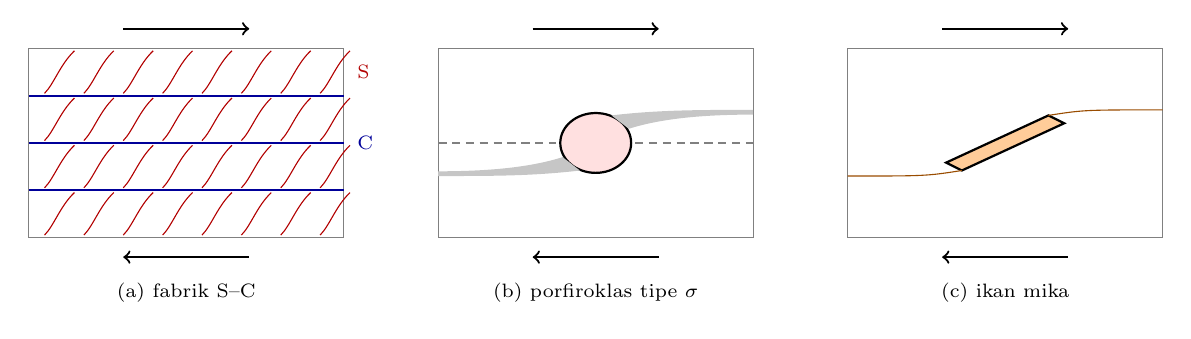
\begin{tikzpicture}[font=\scriptsize, x=1cm, y=1cm]
% (a) S-C fabric, dextral
\begin{scope}
\draw[gray] (0,0) rectangle (4,2.4);
\foreach \y in {0.6,1.2,1.8} {\draw[blue!60!black, thick] (0,\y) -- (4,\y);}
\foreach \y in {0,0.6,1.2,1.8} {\foreach \x in {0.2,0.7,...,3.8} {
  \draw[red!70!black] (\x,\y+0.03) .. controls (\x+0.12,\y+0.15) and (\x+0.2,\y+0.4) .. (\x+0.38,\y+0.57);}}
\draw[->, thick] (1.2,2.65) -- (2.8,2.65);
\draw[<-, thick] (1.2,-0.25) -- (2.8,-0.25);
\node[anchor=north] at (2,-0.45) {(a) fabrik S--C};
\node[blue!60!black, anchor=west] at (4.05,1.2) {C};
\node[red!70!black, anchor=west] at (4.05,2.1) {S};
\end{scope}
% (b) sigma clast
\begin{scope}[shift={(5.2,0)}]
\draw[gray] (0,0) rectangle (4,2.4);
\fill[red!12] (2.0,1.2) ellipse (0.45 and 0.38);
\draw[thick] (2.0,1.2) ellipse (0.45 and 0.38);
\fill[gray!45] (2.2,1.55) .. controls (2.8,1.62) and (3.3,1.62) .. (4.0,1.62) -- (4.0,1.56) .. controls (3.3,1.56) and (2.8,1.5) .. (2.42,1.38) -- cycle;
\fill[gray!45] (1.8,0.85) .. controls (1.2,0.78) and (0.7,0.78) .. (0,0.78) -- (0,0.84) .. controls (0.7,0.84) and (1.2,0.9) .. (1.58,1.02) -- cycle;
\draw[gray, densely dashed] (0,1.2) -- (1.5,1.2) (2.5,1.2) -- (4,1.2);
\draw[->, thick] (1.2,2.65) -- (2.8,2.65);
\draw[<-, thick] (1.2,-0.25) -- (2.8,-0.25);
\node[anchor=north] at (2,-0.45) {(b) porfiroklas tipe $\sigma$};
\end{scope}
% (c) mica fish
\begin{scope}[shift={(10.4,0)}]
\draw[gray] (0,0) rectangle (4,2.4);
\fill[orange!40] (1.25,0.95) -- (2.55,1.55) -- (2.75,1.45) -- (1.45,0.85) -- cycle;
\draw[thick] (1.25,0.95) -- (2.55,1.55) -- (2.75,1.45) -- (1.45,0.85) -- cycle;
\draw[orange!60!black] (2.55,1.55) .. controls (3.0,1.62) .. (4.0,1.62);
\draw[orange!60!black] (1.45,0.85) .. controls (1.0,0.78) .. (0,0.78);
\draw[->, thick] (1.2,2.65) -- (2.8,2.65);
\draw[<-, thick] (1.2,-0.25) -- (2.8,-0.25);
\node[anchor=north] at (2,-0.45) {(c) ikan mika};
\end{scope}
\end{tikzpicture}

\par\smallskip{\small Tiga \omterm{def:b3:deformation-mechanisms:kinematic}{indikator kinematik} dari geser dekstral yang sama
(atas ke kanan, panah), diamati pada bidang lineasi, tegak lurus terhadap
foliasi. (a) Foliasi S (merah) melengkung menjadi pita geser C (biru),
condong ke arah peregangan. (b) Ekor klas tipe $\sigma$
meninggalkan sisi atasnya ke kanan dan sisi bawahnya ke kiri, berpindah naik
searah geser tanpa memotong garis tengah (putus-putus). (c) \omterm{def:b3:deformation-mechanisms:kinematic}{Ikan
mika} condong seperti S, ekornya berpindah seperti ekor klas tipe $\sigma$. Tidak
sesuai skala.}\label{fig:b3:deformation-mechanisms:kinematic}
\end{omfigure}

Jika dibaca bersama, beberapa indikator yang saling sepakat memberi \omterm{def:b3:deformation-mechanisms:kinematic}{arah geser} dengan
keyakinan tinggi; satu indikator saja dapat menyesatkan, karena ada klas yang terotasi balik dan
lipatan asimetris dari asal lain. Foto pada kotak di bawah memperlihatkan
porfiroklas dalam milonit.

\begin{inthelab}[Memeras batuan pada kondisi mantel]
\begin{minipage}[t]{0.55\linewidth}\vspace{0pt}
Dalam alat deformasi bermedium gas, silinder batuan atau bubuk olivin yang dipres panas
panjangnya satu atau dua sentimeter, disegel dalam selubung logam tipis dan
ditempatkan bersama pistonnya di dalam tungku, di dalam bejana baja yang diisi
gas inert terkompresi yang menetapkan tekanan pengekang, beberapa ratus
megapascal. Sebuah aktuator menggerakkan piston pada laju konstan, atau di bawah
beban konstan, sementara sel beban internal mengukur tegangan pada sampel itu sendiri,
bebas dari gesekan segel. Olivin dideformasi dengan cara ini pada
suhu mendekati \qty{1200}{\celsius}; pada akhir percobaan sampel
didinginkan cepat, dipotong, dipoles, lalu diperiksa di bawah mikroskop dan mikroskop elektron,
tempat ukuran butir, \omterm{def:b3:deformation-mechanisms:recrystallisation}{subbutir}, dan \omterm{def:b3:deformation-mechanisms:dislocation}{dislokasinya} diukur.
\end{minipage}\hfill
\begin{minipage}[t]{0.42\linewidth}\vspace{0pt}
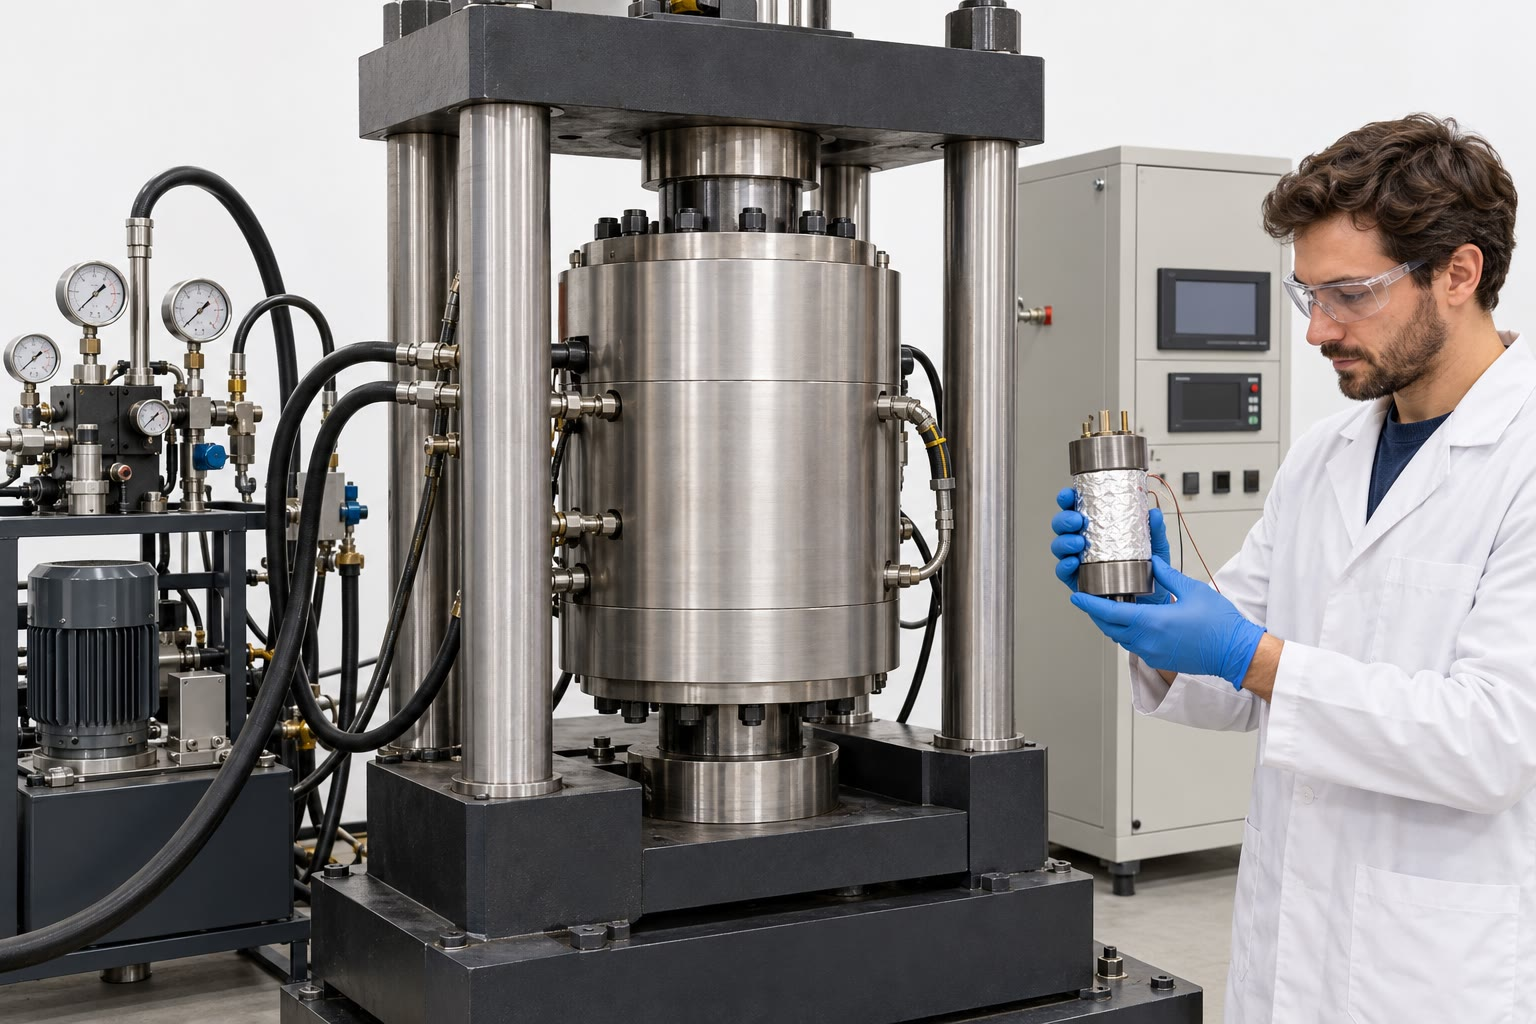
\includegraphics[width=\linewidth]{images/book5/ai/b3-deformation-press.jpg}

{\scriptsize Sebuah pers deformasi batuan dengan rakitan sampel berselubung
(ilustrasi buatan AI).}

\smallskip
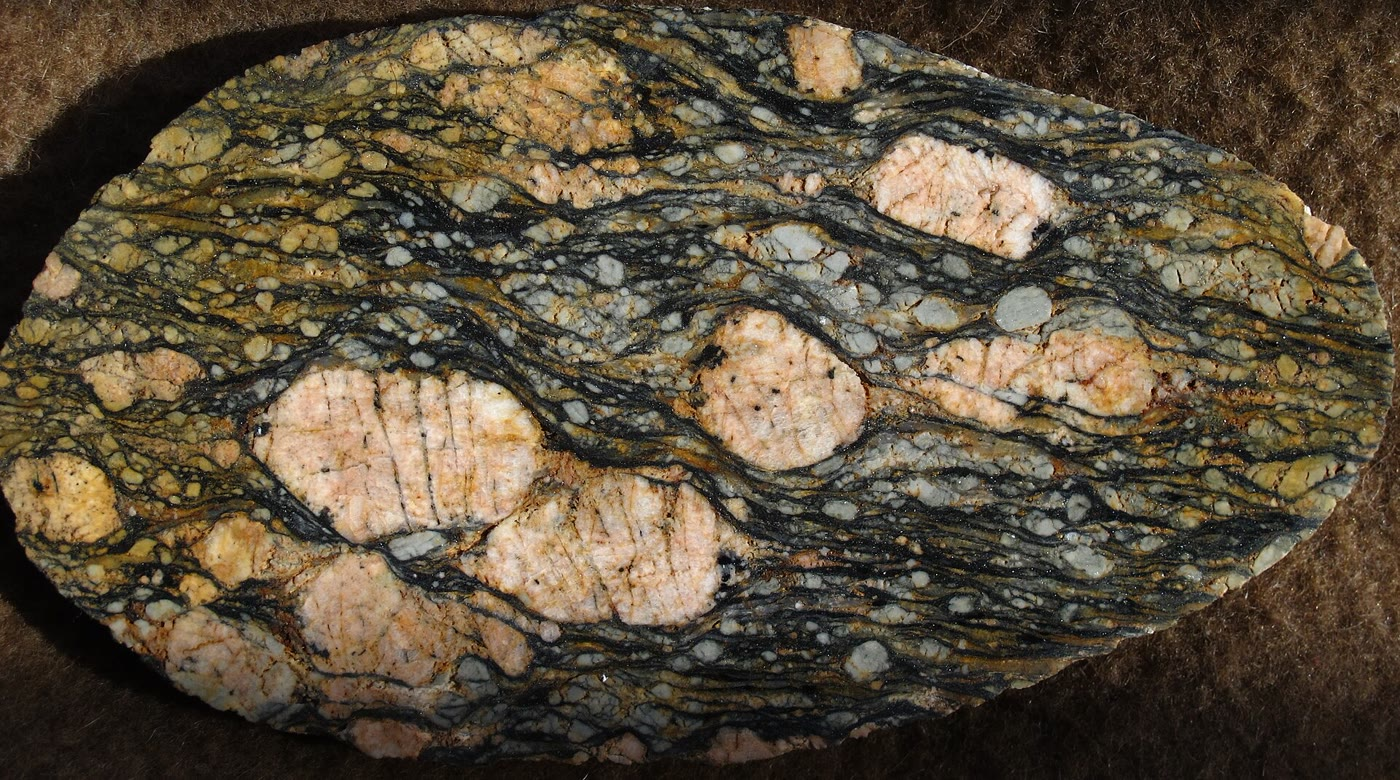
\includegraphics[width=\linewidth]{images/book5/b3-augen-mylonite.jpg}

{\scriptsize Milonit augen yang digergaji dari Norwegia: porfiroklas feldspar besar
dalam matriks halus kuarsa, feldspar, dan mika hasil rekristalisasi. Foto
Mikenorton, CC BY-SA 4.0.}
\end{minipage}
\end{inthelab}
% ledger: mk00:diffusion, photo:b3-augen-mylonite

\section{Latihan}

\begin{exercise}[$\star$]\label{exo:b3:deformation-mechanisms:1}
Forsterit meleleh pada \qty{1890}{\celsius} dan es pada \qty{0}{\celsius}. Hitung
\omterm{def:b3:deformation-mechanisms:flow-law}{suhu homolog} forsterit pada \qty{1300}{\celsius} dan es pada
\qty{-10}{\celsius}. Mana yang lebih mudah merayap?
\end{exercise}

\begin{exercise}[$\star$]\label{exo:b3:deformation-mechanisms:2}
Sebuah retas yang memotong \omterm{def:b3:deformation-mechanisms:shear-zone}{zona geser} tegak lurus dibelokkan di dalam zona itu
sebesar \ang{70}, dan retas lain sebesar \ang{80}. Hitung regangan geser. Mengapa
regangan besar sulit diukur dengan cara ini?
\end{exercise}

\begin{exercise}[$\star$]\label{exo:b3:deformation-mechanisms:3}
Dengan piezometer kuarsa, tegangan apa yang ditunjukkan oleh ukuran butir hasil
rekristalisasi sebesar \qty{10}{\micro m}?
\end{exercise}

\begin{exercise}[$\star$]\label{exo:b3:deformation-mechanisms:4}
Dengan \omterm{def:b3:deformation-mechanisms:flow-law}{hukum aliran} kuarsit basah ($A = \num{1.1e-4}$, $n = 4$, $E =
\qty{223}{kJ.mol^{-1}}$, $R = \qty{8.314}{J.mol^{-1}.K^{-1}}$), hitung
laju regangan pada \qty{500}{\celsius} di bawah \qty{20}{MPa}.
\end{exercise}

\begin{exercise}[$\star\star$]\label{exo:b3:deformation-mechanisms:5}
Hitung viskositas efektif kuarsit basah yang mengalir pada \qty{e-14}{s^{-1}}
pada \qty{400}{\celsius} (\qty{65.4}{MPa}) dan pada \qty{500}{\celsius}
(\qty{18.0}{MPa}). Bandingkan dengan \omterm{def:b3:mantle-convection:gia}{viskositas mantel} pada
\cref{ch:b3:mantle-convection}.
\end{exercise}

\begin{exercise}[$\star\star$]\label{exo:b3:deformation-mechanisms:6}
Dua percobaan pada suhu yang sama menghasilkan \qty{e-5}{s^{-1}} di bawah
\qty{100}{MPa} dan \qty{1.6e-4}{s^{-1}} di bawah \qty{200}{MPa}. Hitung \omterm{def:b3:deformation-mechanisms:flow-law}{eksponen tegangan}
dan sebutkan mekanisme yang paling mungkin.
\end{exercise}

\begin{exercise}[$\star\star$]\label{exo:b3:deformation-mechanisms:7}
Pada tegangan yang sama, sebuah sampel merayap sepuluh kali lebih cepat pada \qty{1100}{K} daripada
pada \qty{1000}{K}. Hitung energi aktivasi.
\end{exercise}

\begin{exercise}[$\star\star$]\label{exo:b3:deformation-mechanisms:8}
Dengan faktor berapa laju regangan \omterm{def:b3:deformation-mechanisms:creep}{rayapan difusi} berubah ketika ukuran butir
dibagi sepuluh, untuk rayapan Nabarro--Herring dan untuk rayapan Coble? Mengapa
rayapan Coble lebih sensitif?
\end{exercise}

\begin{exercise}[$\star\star$]\label{exo:b3:deformation-mechanisms:9}
Untuk olivin kering pada \qty{1100}{\celsius} dan \qty{2}{GPa}, kedua \omterm{def:b3:deformation-mechanisms:flow-law}{hukum aliran}
$\dot\varepsilon_{\mathrm{dis}} = \num{6.54e-17}\,\sigma^{3.5}$ dan
$\dot\varepsilon_{\mathrm{dif}} = \num{3.59e-6}\,\sigma d^{-3}$ (satuan seperti dalam
teks). Hitung tegangan batas untuk $d = \qty{1}{mm}$ dan $d =
\qty{100}{\micro m}$, serta kemiringan batasnya.
\end{exercise}

\begin{exercise}[$\star\star\star$]\label{exo:b3:deformation-mechanisms:10}
Mengikuti pembuktian \cref{prop:b3:deformation-mechanisms:grain-size},
jelaskan mengapa jalur kisi memberikan $d^{-2}$ dan jalur batas memberikan $d^{-3}$, serta
tunjukkan bahwa difusi batas mendominasi di bawah ukuran butir $d^* \approx
(B_B/B_L)\,\delta D_B/D_L$.
\end{exercise}

\begin{exercise}[$\star\star\star$]\label{exo:b3:deformation-mechanisms:11}
Untuk \omterm{def:b3:deformation-mechanisms:flow-law}{hukum aliran} dengan $n = 3.5$, dengan faktor berapa viskositas efektif turun
ketika laju regangan dikalikan sepuluh? Mengapa hal ini memihak
lokalisasi regangan ke dalam \omterm{def:b3:deformation-mechanisms:shear-zone}{zona geser}?
\end{exercise}

\begin{exercise}[$\star\star\star$]\label{exo:b3:deformation-mechanisms:12}
Pada olivin kering pada soal 9, \omterm{def:b3:deformation-mechanisms:shear-zone}{zona geser} mantel di bawah \qty{10}{MPa}
mengalami rekristalisasi dari butir \qty{3}{mm} menjadi butir \qty{30}{\micro m}. Hitung
laju regangan total sebelum dan sesudah, serta faktor pelunakannya. Mekanisme mana
yang menanggung deformasi pada tiap kasus?
\end{exercise}

\section{Soal: Zona geser Varden}

\begin{problem}[{Soal akhir pekan --- regangan, tegangan, laju regangan, dan umur
zona geser fiktif}]
\label{pb:b3:deformation-mechanisms:1}
% values: calc/ch07.py; flow_laws.py; st03:piezometer, lopez:flow-laws
Di bawah granit Bukit Varden, wilayah fiktif rangkaian ini, sebuah
sumur bor dan sayatan jalan dalam (keduanya fiktif) memperlihatkan \omterm{def:b3:deformation-mechanisms:shear-zone}{zona geser} duktil
selebar \qty{400}{m}, terbentuk pada kedalaman sekitar \qty{15}{km} dan suhu \qty{450}{\celsius}.
Sebuah retas dolerit yang memotong dinding tegak lurus membentuk, di dalam zona itu,
sudut hanya \ang{6} dengan batas zona. Kuarsanya adalah milonit
dari butir hasil rekristalisasi selebar \qty{20}{\micro m} (dari 15 sampai
\qty{25}{\micro m}). Gunakan piezometer kuarsa $D = 10^{3.56}\sigma^{-1.26}$,
\omterm{def:b3:deformation-mechanisms:flow-law}{hukum aliran} kuarsit basah ($A = \num{1.1e-4}$, $n = 4$, $E =
\qty{223}{kJ.mol^{-1}}$), $R = \qty{8.314}{J.mol^{-1}.K^{-1}}$, \qty{1}{yr} $=
\qty{3.156e7}{s}$, dan, pada geser sederhana, $\dot\gamma = 2\dot\varepsilon$.

\medskip\noindent\textbf{Bagian I --- Regangan.}
\begin{enumerate}
  \item Hitung defleksi $\psi$ dari retas dan regangan gesernya.
  \item Hitung pergeseran satu dinding terhadap dinding lainnya.
  \item Hitung peregangan utama elips regangan dan rasio
        aksialnya.
  \item Hitung sudut sumbu panjang terhadap zona. Apa yang
        dilakukan foliasi zona ketika $\gamma$ membesar?
  \item Dilihat dari atas, retas yang ditelusuri dari dinding selatan
        membelok ke timur ketika memasuki zona timur--barat, lalu kembali
        ke jalur utaranya di dinding utara. Ke arah mana dinding utara
        bergerak, dan apakah zona itu dekstral atau sinistral?
  \item Pada bidang mana sayatan tipis harus dipotong untuk membaca
        \omterm{def:b3:deformation-mechanisms:kinematic}{indikator kinematik}, dan bagaimana foliasi S-nya seharusnya miring?
\end{enumerate}

\medskip\noindent\textbf{Bagian II --- Tegangan.}
\begin{enumerate}[resume]
  \item Hitung tegangan yang ditunjukkan oleh butir \qty{20}{\micro m}.
  \item Hitung tegangan untuk ukuran 15 dan \qty{25}{\micro m}.
  \item Apakah tegangan berada dalam rentang kalibrasi?
  \item Piezometer tidak menunjukkan pengaruh suhu. Mengapa hal ini penting
        di sini?
  \item Ukuran butir berapa yang akan dihasilkan oleh tegangan \qty{100}{MPa}?
\end{enumerate}

\medskip\noindent\textbf{Bagian III --- Laju regangan.}
\begin{enumerate}[resume]
  \item Hitung $E/RT$ pada \qty{450}{\celsius} dan faktor Arrhenius.
  \item Hitung laju regangan kuarsa di bawah tegangan pada pertanyaan 7
        (gunakan \qty{62}{MPa}).
  \item Hitung laju regangan geser.
  \item Hitung viskositas efektif zona dan bandingkan dengan
        mantel atas pada \cref{ch:b3:mantle-convection}.
  \item Dengan faktor berapa laju regangan berubah pada 400 dan
        \qty{500}{\celsius}, dengan tegangan yang sama?
  \item Dengan faktor berapa jika tegangannya \qty{78}{MPa}, nilai untuk
        butir paling halus?
\end{enumerate}

\medskip\noindent\textbf{Bagian IV --- Waktu.}
\begin{enumerate}[resume]
  \item Hitung waktu yang dibutuhkan untuk mengumpulkan regangan geser pada pertanyaan 1,
        dalam detik.
  \item Konversikan ke ribuan tahun.
  \item Hitung laju geser rata-rata sepanjang zona, dalam \unit{mm/yr}.
  \item Bandingkan dengan laju batas lempeng yang berorde puluhan milimeter per tahun.
        % ledger: morvel:range
  \item Jika zona itu memiliki laju \qty{20}{mm/yr}, berapa laju regangan geser, tegangan
        dan ukuran butir hasil rekristalisasi yang akan dimilikinya?
  \item Bagaimana ketidakpastian ukuran butir dan \omterm{def:b3:deformation-mechanisms:flow-law}{eksponen tegangan}
        piezometer memengaruhi waktu?
  \item Berikan waktu yang dibutuhkan \omterm{def:b3:deformation-mechanisms:shear-zone}{zona geser} Varden untuk mengumpulkan regangannya, dalam
        ribuan tahun.
\end{enumerate}
\end{problem}
